\documentclass[prb,12pt]{revtex4-2}
%fonts
% Palatino for main text and math
\usepackage[osf,sc]{mathpazo}

% Helvetica for sans serif
% (scaled to match size of Palatino)
\usepackage[scaled=0.90]{helvet}

% Bera Mono for monospaced
% (scaled to match size of Palatino)
\usepackage[scaled=0.85]{beramono}
\usepackage{amsmath, amssymb,physics,amsfonts,amsthm}
\usepackage{enumitem}
\usepackage{cancel}
\usepackage[most]{tcolorbox}
\usepackage{booktabs}
\usepackage{tikz}
\usepackage{hyperref}
\usepackage{enumitem}
\usepackage{transparent}
\usepackage{float}
\usepackage{multirow}
\newtheorem{Theorem}{Theorem}
\newtheorem{Proposition}{Proposition}
\newtheorem{Lemma}[Theorem]{Lemma}
\newtheorem{Corollary}[Theorem]{Corollary}
\newtheorem{Example}[Theorem]{Example}
\newtheorem{Remark}[Theorem]{Remark}
\theoremstyle{definition}
\newtheorem{Problem}{Problem}
\theoremstyle{definition}
\newtheorem{Definition}[Theorem]{Definition}
\newenvironment{parts}{\begin{enumerate}[label=(\alph*)]}{\end{enumerate}}
%tikz
\usetikzlibrary{patterns}
\usepackage{tikz-cd}
% definitions of number sets
\newcommand{\N}{\mathbb{N}}
\newcommand{\R}{\mathbb{R}}
\newcommand{\Z}{\mathbb{Z}}
\newcommand{\Q}{\mathbb{Q}}
\newcommand{\C}{\mathbb{C}}
\allowdisplaybreaks

\newtcolorbox{revision}[1][]{empty, breakable, sharp corners, borderline north={1pt}{0pt}{black},
	borderline west={5pt}{0pt}{black},
	#1}

\begin{document}
	\title{Algebra und Dynamik von Quantensystemen Blatt Nr. 1}
	\author{Jun Wei Tan}
	\email{jun-wei.tan@stud-mail.uni-wuerzburg.de}
	\affiliation{Julius-Maximilians-Universit\"{a}t W\"{u}rzburg}
	\date{\today}
	\maketitle
\paragraph{Aufgabe 1.1}
\begin{parts}
	\item 
		\begin{center}
			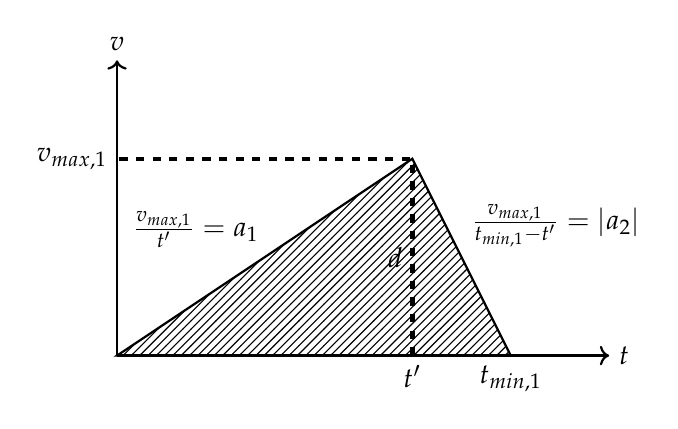
\begin{tikzpicture}[scale=2.5]
				\draw[thick, ->] (0,0) -- (2.5,0);
			\draw[thick, ->] (0,0) -- (0,1.5);
			\filldraw[thick, pattern = north east lines] (0,0) -- (1.5,1) -- (2,0) -- cycle;
			\draw (0,1.5) node[anchor=south] {$v$};
			\draw (2.5,0) node[anchor=west] {$t$};
			\draw (2,0) node[anchor=north] {$t_{min,1}$};
			\draw[ultra thick, dashed] (1.5,0) -- (1.5,1) -- (0,1);
			\draw (0,1) node[anchor=east] {$v_{max,1}$};
			\draw (1.5,0) node[anchor=north] {$t'$};
			\draw (0.4,0.5) node[anchor=south] {$\frac{v_{max,1}}{t'}=a_1$};
			\draw (1.75,0.5) node[anchor=south west] {$\frac{v_{max,1}}{t_{min,1}-t'} = |a_2|$};
			\draw (1.5,0.5) node[anchor=east] {$d$};
			\end{tikzpicture}
		\end{center}
		Man löst die Gleichungen
		\begin{align}
			\frac{1}{2}(v_{max,1})(t_{min,1})=&d\label{eqn1}\\
			v_{max,1}=&a_1t'\label{eqn2}\\
			v_{max,1}=&(t'-t_{min,1})a_2\label{eqn3}
		\end{align}
		Aus \eqref{eqn2} folgt $t'=v_{max,1} / a_1$. Wir setzen das in \eqref{eqn3} ein. Es ergibt sich
		\[
			v_{max,1}=\left( \frac{v_{max,1}}{a_1}-t_{min,1} \right) a_2
		.\] 
		Daraus folgt:
		\[
			v_{max,1}\left( 1-\frac{a_2}{a_1} \right) =-t_{min,1}a_2
		.\] 
	\item 	Noch einmal setzen wir das in \eqref{eqn1} ein:
		\[
			\frac{1}{2}\left[ -t_{min,1}a_2\left( 1-\frac{a_2}{a_1} \right)^{-1} \right] \left( t_{min,1} \right) =d 
		.\] 
		Die L\"{o}sung ist
		\[
			t_{min,1}=\boxed{\left[ -\frac{2d}{a_2}\left( 1-\frac{a_2}{a_1} \right)  \right]^{1 / 2}}
		.\] 
		Aus \eqref{eqn1} folgt
		\[
			v_{max,1}=\frac{2d}{t_{mn,1}}
		.\] 
		Also
		\[
			v_{max,1}=\boxed{\left[ -\frac{1-\frac{a_2}{a_1}}{2a_2d} \right]^{-1 / 2}} 
		.\] 
	\item 
		\begin{center}
			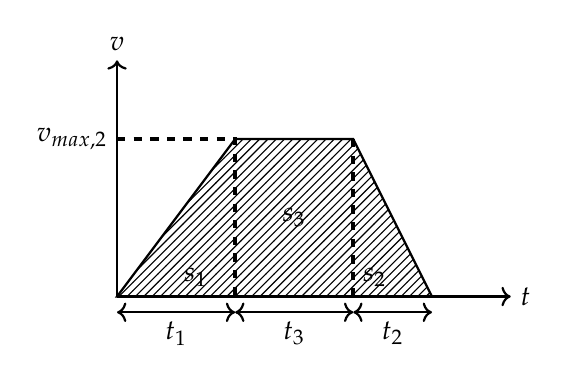
\begin{tikzpicture}[scale=2]
				\draw[thick, ->] (0,0) --(2.5,0);
				\draw[thick, ->] (0,0) -- (0,1.5);
				\filldraw[thick,pattern = north east lines] (0,0) -- (0.75,1) -- (1.5,1) -- (2,0) -- cycle;
				\draw[ultra thick, dashed] (0,1) -- (0.75,1) -- (0.75,0);
				\draw[ultra thick, dashed] (1.5,1) -- (1.5,0);
				\draw (0,1) node[anchor=east] {$v_{max,2}$};
				\draw[thick, <->] (0,-0.1) -- (0.75,-0.1);
				\draw (0.375,-0.1) node[anchor=north] {$t_1$};
				\draw (2.5,0) node[anchor=west] {$t$};
				\draw[thick,<->] (1.5,-0.1) -- (2,-0.1);
				\draw (1.75,-0.1) node[anchor=north] {$t_2$};
				\draw (0,1.5) node[anchor=south] {$v$};
				\draw (0.5,0) node[anchor=south] {$s_1$};
				\draw (1.5,0) node[anchor=south west] {$s_2$};
				\draw (1.125,0.5) node {$s_3$};
				\draw[thick,<->] (0.75,-0.1) -- (1.5,-0.1);
				\draw (1.125,-0.1) node[anchor=north] {$t_3$};
			\end{tikzpicture}
		\end{center}
		Es gilt
		\begin{align*}
			t_1=&\frac{v_{max,2}}{a_1}\\
			t_2=&-\frac{v_{max,2}}{a_2}\\
			s_1=&\frac{1}{2}a_1t_1^2=\frac{v_{max,2}^2}{2a_1}\\
			s_2=&\frac{1}{2}v_{max,2}t_2=-\frac{v_{max,2}^2}{2a_2}\\
			s_3=&v_{max,2}t_3=d-s_1-s_2\\
			t_3=&\frac{d-s_1-s_2}{v_{max,2}}\\
			=&\frac{d}{v_{max,2}}-\frac{v_{max,2}}{2a_1}+\frac{v_{max,2}}{2a_2}\\
			t_{min,2}=&t_1+t_2+t_3\\
			=&\frac{d}{v_{max,2}}+\frac{v_{max,2}}{2a_1}-\frac{v_{max,2}}{2a_2}\\
		\end{align*}

\end{parts}
\paragraph{Aufgabe 1.2}
\begin{center}
	\begin{tikzpicture}[scale=2.5]
		\draw[thick, ->] (0,0) -- (0,{(3-sqrt(3))/(1+sqrt(3))});
		\draw[thick, ->] (0,{(3-sqrt(3))/(1+sqrt(3))}) -- ++({0.4*cos(60)},{0.4*sin(60)});
		\draw (0,{(3-sqrt(3))/(2*(1+sqrt(3)))}) node[anchor=east] {$h_0$};
		\draw[thick, ->] (2,0) -- (2,1);\draw (2,0.5) node[anchor=west] {$h_1$};
		\draw[thick] (0,{(3-sqrt(3))/(1+sqrt(3))}) arc (150:60:{4/(1+sqrt(3))});
		\draw[thick,<->] (0,0) -- (2,0);
		\draw (1,0) node[anchor=north] {$l$};
	\end{tikzpicture}
\end{center}
\begin{gather*}
	x=v_0t\cos\theta\\
	y=v_0t\sin\theta-\frac{1}{2}gt^2\\
	y=x\tan\theta-\frac{gx^2}{2v_0^2\cos^2\theta}
\end{gather*}
Wir brauchen $y(l)=h_1-h_0$, oder
\[
h_1-h_0=l\tan\theta-\frac{gl^2}{2v_0^2\cos^2\theta}
.\] 
Daraus folgt
\[
v_0^2=\frac{gl^2}{2\cos^2\theta\left( l\tan\theta-(h_1-h_0) \right) }
.\] 

\begin{center}
	$l=h_1=1\text{ m},h_0=0\text{ m}$


	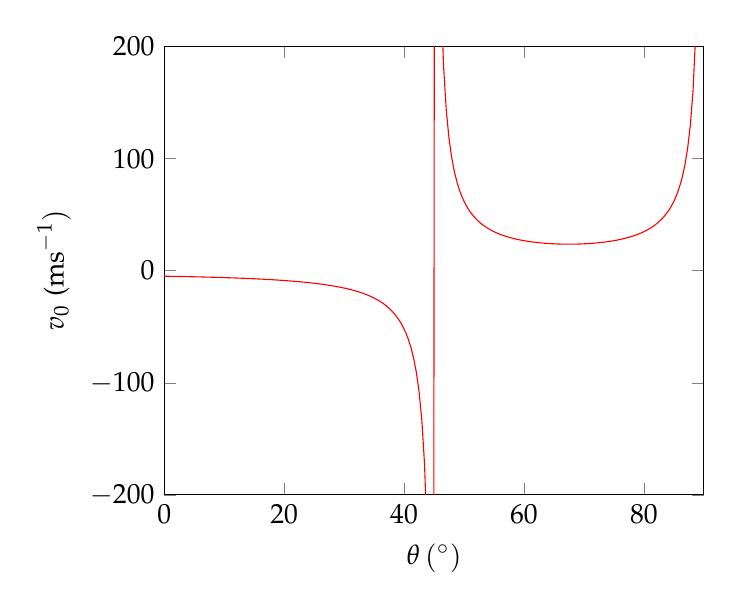
\begin{tikzpicture}
		\begin{axis}[ymin=-200,ymax=200,xmin=0,xmax=90,xlabel=$\theta\left( ^{\circ} \right) $,ylabel=$v_0\text{ (ms}^{-1})$]
\addplot[domain=0:90,color=red,samples=200]{9.81/(2*cos(x)*cos(x)*(tan(x)-1))};
\end{axis}
	\end{tikzpicture}
\end{center}
Es folgt daraus:
\[
y=x\tan\theta-(l\tan\theta-(h_1-h_0))\frac{x^2}{l^2}
.\] 
\paragraph{Aufgabe 1.3}
\begin{center}
	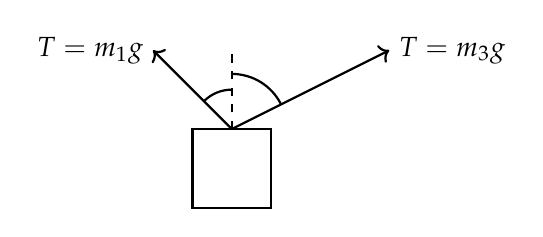
\begin{tikzpicture}
		\draw[thick] (-0.5,-1) rectangle (0.5,0);
		\draw[thick,->] (0,0) -- (-1,1);
		\draw[thick,->] (0,0) -- (2,1);
		\draw[thick, dashed] (0,0) -- (0,1);
		\draw[thick] (0,0.5) arc(90:135:0.5);
		\draw[thick] (0,0.7) arc(90:{atan(0.5)}:0.7);
		\draw (-1,1) node[anchor=east] {$T=m_1g$};
		\draw (2,1) node[anchor=west] {$T=m_3g$};
	\end{tikzpicture}
\end{center}
Es gilt
\begin{align*}
	x:& m_1g\sin\alpha=m_3g\sin\beta\\
	y:& m_1g\cos\alpha+m_3g\cos\beta=m_2g
\end{align*}
Also
\begin{align*}
	m_3=&m_1\frac{\sin\alpha}{\sin\beta}\\
	m_1\cos\alpha+m_1\frac{\sin\alpha}{\sin\beta}\cos\beta=&m_2\\
	m_1=&\frac{m_2}{\cos\alpha+\cos\beta\left( \frac{\sin\alpha}{\sin\beta} \right) }\\
	=& \frac{m_2\sin\beta}{\sin(\alpha+\beta)}\\
	m_3=&\frac{m_2\sin\alpha}{\sin(\alpha+\beta)}
\end{align*}
\begin{center}
	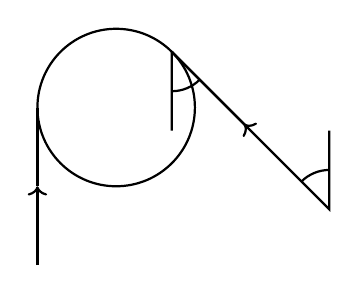
\begin{tikzpicture}
		\draw[thick] (0,0) circle (1);
		\draw[thick,->] (-1,-2) -- (-1,-1);
		\draw[thick] (-1,-1) -- (-1,0);
		\draw[thick,-<] ({1/sqrt(2)},{1/sqrt(2)}) -- ++(1,-1);
		\draw[thick] ({1/sqrt(2)},{1/sqrt(2)}) -- ++(2,-2) -- ++(0,1) -- ++(0,-0.5) arc(90:135:0.5);
		\draw[thick] ({1/sqrt(2)},{1/sqrt(2)}) -- ++(0,-1) -- ++(0,0.5) arc(-90:-45:0.5);
	\end{tikzpicture}
\end{center}
\begin{align*}
	\va F=&-\left[ \begin{pmatrix} 0 \\ -m_1g \end{pmatrix} +m_1g\begin{pmatrix} \sin\alpha \\-\cos\alpha  \end{pmatrix}  \right]\\
	=& m_1g\begin{pmatrix} -\sin\alpha \\ 1+\cos\alpha \end{pmatrix} 
\end{align*}
\paragraph{Aufgabe 1.4}
\begin{parts}
\item 
\noindent \\
	\begin{center}
		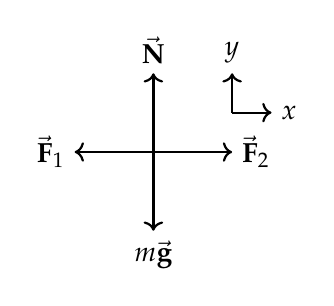
\begin{tikzpicture}
			\draw[thick,->] (0,0) -- (1,0);
			\draw (1,0) node[anchor=west] {$\va F_2$};
			\draw[thick, ->] (0,0) -- (-1,0);
			\draw (-1,0) node[anchor=east] {$\va F_1$};
			\draw[thick,->] (0,0) -- (0,1);
			\draw (0,1) node[anchor=south] {$\va N$};
			\draw (0,-1) node[anchor=north] {$m\va g$};
			\draw[thick, ->] (0,0) -- (0,-1);
			\draw[thick,->]	 (1,0.5) -- (1,1);
			\draw[thick, ->] (1,0.5) -- (1.5,0.5);
			\draw (1,1) node[anchor=south] {$y$};
			\draw (1.5,0.5) node[anchor=west] {$x$};
		\end{tikzpicture}
	\end{center}
\item $a_y=0$ (Zwangsbedingung), $a_x=\frac{1}{3m}\left(|F_2|-|F_1|\right)$
\item \noindent \\
	\begin{center}
		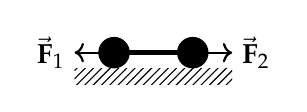
\begin{tikzpicture}[scale=1]
			\fill[pattern = north east lines] (0,-0.2) rectangle (2,0);
		\fill (0.5,0.2) circle (0.2);
	\fill (1.5,0.2) circle (0.2);
	\draw[thick, ->] (0.5,0.2) -- (0,0.2);
	\draw[thick, ->] (1.5,0.2) -- (2,0.2);
	\draw (0,0.2) node[anchor=east] {$\va F_1$};
	\draw (2,0.2) node[anchor=west] {$\va F_2$};
	\draw[ultra thick] (0.5,0.2) -- (1.5,0.2);
		\end{tikzpicture}
	\end{center}
	\[
	a_1=a_2=\frac{1}{3m}\left(|\va F_2|-|\va F_1| \right) 
	.\] 
\item \noindent \\
	\begin{center}
		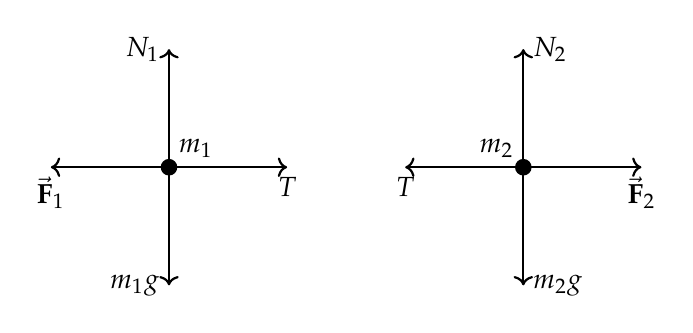
\begin{tikzpicture}[scale=1.5]
		\fill (0,0) circle (2pt);
		\draw[thick, ->] (0,0) -- (1,0);
		\draw[thick, ->] (0,0) -- (0,1);
		\draw[thick, ->] (0,0) -- (-1,0);
		\draw[thick, ->] (0,0) -- (0,-1);
	\fill (3,0) circle (2pt);
	\draw[thick, ->] (3,0) -- (4,0);
	\draw[thick, ->] (3,0) -- (3,1);
	\draw[thick, ->] (3,0) -- (3,-1); 
	\draw[thick, ->] (3,0) -- (2,0);
	\draw (1,0) node[anchor=north] {$T$};
	\draw (0,1) node[anchor=east] {$N_1$};
	\draw (0,-1) node[anchor=east] {$m_1g$};
	\draw (-1,0) node[anchor=north] {$\va F_1$};
	\draw (4,0) node[anchor=north] {$\va F_2$};
	\draw (2,0) node[anchor=north] {$T$};
	\draw (3,1) node[anchor=west] {$N_2$};
	\draw (3,-1) node[anchor=west] {$m_2g$};
	\draw (0,0) node[anchor=south west] {$m_1$};
	\draw (3,0) node[anchor=south east] {$m_2$};
		\end{tikzpicture}
	\end{center}
\item 
	\begin{align*}
		m_1a=&T-F_1\\
		m_2a=& F_2-T\\
		(m_1+m_2)a=&T-F_1+F_2-T\\
		=&F_2-F_1\\
		=&3ma\\
		a=&\frac{1}{3m}\left( F_2-F_1 \right) 
	\end{align*}
\end{parts}


\end{document}
